%Este trabalho está licenciado sob a Licença Atribuição-CompartilhaIgual 4.0 Internacional Creative Commons. Para visualizar uma cópia desta licença, visite http://creativecommons.org/licenses/by-sa/4.0/deed.pt_BR ou mande uma carta para Creative Commons, PO Box 1866, Mountain View, CA 94042, USA.

\chapter{Produto escalar}\label{cap_prodesc}
\thispagestyle{fancy}

\section{Produto escalar}\label{cap_prodesc_sec_prodesc}

Ao longo desta seção, assumiremos $B = (\vec{i},\vec{j},\vec{k})$ uma base ortonormal no espaço\footnote{$(\vec{i},\vec{j},\vec{k})$ é l.i., $|\vec{i}|=1$, $|\vec{j}|=1$, $|\vec{k}|=1$ e dois a dois ortogonais. Veja Subseção \ref{subsec:cbsbc_bortonormal}.}. Por simplicidade de notação, vamos denotar as coordenas de um vetor $\vec{u}$ na base $B$ por
\begin{equation}
  \vec{u} = (u_1, u_2, u_3),
\end{equation}
i.e. $\vec{u} = u_1\vec{i} + u_2\vec{j} + u_3\vec{k}$.

O {\color{blue}\bf produto escalar} dos vetores $\vec{u} = (u_1,u_2,u_3)$ e $\vec{v}=(v_1,v_2,v_3)$ é o número real
\begin{equation}\label{eq:prodesc_ortonormal}
  {\color{blue}\vec{u}\cdot\vec{v} = u_1v_1+u_2v_2+u_3v_3}.
\end{equation}

\begin{ex}
  Se $\vec{u}=(2,-1,3)$ e $\vec{v}=(-3,-4,2)$, então
  \begin{equation}
    \vec{u}\cdot\vec{v} = 2\cdot(-3)+(-1)\cdot(-4)+3\cdot 2 = 4.
  \end{equation}
\end{ex}

\subsection{Propriedades do produto escalar}

Quaisquer que sejam $\vec{u}$, $\vec{v}$, $\vec{w}$ e qualquer número real $\alpha$, temos:
\begin{itemize}
\item {\bf Comutatividade:}
  \begin{equation}
    {\color{blue}\vec{u}\cdot\vec{v}=\vec{v}\cdot\vec{u}}
  \end{equation}

  Dem.:
  \begin{align}
    \vec{u}\cdot\vec{v} &= (u_1,u_2,u_3)\cdot(v_1,v_2,v_3)\\
                        &= u_1v_1+u_2v_2+u_3v_3 \\
                        &= v_1u_1+v_2u_2+v_3u_3 \\
                        &= \vec{v}\cdot\vec{u}.
  \end{align}

\item {\bf Associatividade com a multiplicação por escalar:}
  \begin{equation}
    {\color{blue}(\alpha\vec{u})\cdot\vec{v}=\vec{u}\cdot(\alpha\vec{v})=\alpha(\vec{u}\cdot\vec{v})}
\end{equation}

  Dem.:
  \begin{align}
    (\alpha\vec{u})\cdot\vec{v} &= (\alpha u_1,\alpha u_2, \alpha u_3)\cdot (v_1,v_2,v_3)\\
                                &= (\alpha u_1)v_1+(\alpha u_2)v_2 + (\alpha u_3)v_3 \\
                                &= \alpha (u_1v_1)+\alpha (u_2v_2)+\alpha (u_3v_3) \\
                                &= \alpha (u_1v_1+u_2v_2+u_3v_3) = \alpha(\vec{u}\cdot\vec{v})\\
                                &= u_1(\alpha v_1) + u_2(\alpha v_2) + u_3(\alpha v_3) \\
                                &= (u_1,u_2,u_3)\cdot(\alpha v_1,\alpha v_2,\alpha v_3) \\
                                &= \vec{u}\cdot(\alpha\vec{v}).
  \end{align}

\item {\bf Distributividade com a adição:}
  \begin{equation}
    {\color{blue}\vec{u}\cdot(\vec{v}+\vec{w}) = \vec{u}\cdot\vec{v}+\vec{u}\cdot\vec{w}}
\end{equation}
  Dem.:
  \begin{align}
    \vec{u}\cdot(\vec{v}+\vec{w}) &= (u_1,u_2,u_3)\cdot\left((v_1,v_2,v_3)+(w_1,w_2,w_3)\right) \\
                                  &= (u_1,u_2,u_3)\cdot [(v_1+w_1,v_2+w_2,v_3+w_3)] \\
                                  &= u_1(v_1+w_1) + u_2(v_2+w_2) + u_2(v_2+w_2) \\
                                  &= u_1v_1+u_1w_1+u_2v_2+u_2w_2+u_3v_3+u_3w_3 \\
                                  &= u_1v_1+u_2v_2+u_3v_3 + u_1w_1+u_2w_2+u_3w_3 \\
                                  &= \vec{u}\cdot\vec{v}+\vec{u}\cdot\vec{w}.
  \end{align}

\item {\bf Sinal:}
  \begin{gather}
    {\color{blue}\vec{u}\cdot\vec{u}\geq 0},\quad\text{e}\\
    {\color{blue}\vec{u}\cdot\vec{u}=0 \Leftrightarrow \vec{u}=\vec{0}}
\end{gather}

  Dem.:
  \begin{align}
    \vec{u}\cdot\vec{u} = u_1^2+u_2^2+u_3^2 \geq 0.
  \end{align}
  Além disso, observamos que a soma de números não negativos é nula se, e somente se, os números forem zeros.

\item {\bf Norma:}
  \begin{equation}
    {\color{blue}|u|^2 = \vec{u}\cdot\vec{u}}
\end{equation}
  Dem.:
  Como fixamos uma base ortonormal $B$, a Proposição \ref{prop:bo_norma} nos garante que
  \begin{equation}
    |u|^2 = u_1^2+u_2^2+u_3^2 = \vec{u}\cdot\vec{u}.
  \end{equation}
\end{itemize}

\begin{ex}
  Sejam $\vec{u}=(-1,2,1)$, $\vec{v}=(2,-1,3)$ e $\vec{w}=(1,0,-1)$. Vejamos se as propriedades se verificam para estes vetores.
  \begin{itemize}
  \item Comutatividade:
    \begin{gather}
      \vec{u}\cdot\vec{v} = -1\cdot 2 + 2\cdot (-1) + 1\cdot 3 = -1\\
      \vec{v}\cdot\vec{u} = 2\cdot(-1) + (-1)\cdot 2 + 3\cdot 1 = -1~\checkmark
    \end{gather}
  \item Associatividade com a multiplicação por escalar:
    \begin{gather}
      (2\vec{u})\cdot\vec{v} = (-2,4,2)\cdot(2,-1,3) = -4-4+6=-2\\
      2(\vec{u}\vec{v}) = 2(-2-2+3) = -2~\checkmark\\
      \vec{u}\cdot(2\vec{v}) = (-1,2,1)\cdot(4,-2,6) = -2~\checkmark
    \end{gather}
  \item Distributividade com a adição:
    \begin{gather}
      \vec{u}\cdot(\vec{v}+\vec{w}) = (-1,2,1)\cdot(3,-1,2) = -3-2+2=-3\\
      \vec{u}\cdot\vec{v}+\vec{u}\cdot\vec{w} = (-2-2+3)+(-1+0-1) = -3~\checkmark
    \end{gather}
  \item Sinal:
    \begin{equation}
      \vec{w}\vec{w} = 1+0+1 = 2 \geq 0~\checkmark
    \end{equation}
  \item Norma:
    \begin{gather}
      |u|^2 = (-1)^2+2^2+1^2 = 6\\
      \vec{u}\cdot\vec{u} = (-1)\cdot(-1)+2\cdot 2+1\cdot 1 = 6~\checkmark
    \end{gather}
  \end{itemize}
\end{ex}

\subsection*{Exercícios resolvidos}

\begin{exeresol}
  Sejam
  \begin{gather}
    \vec{u} = (-1,0,1)\\
    \vec{v} = (0,2,1)\\
    \vec{w} = (2,-1,-1)
  \end{gather}
  calcule $\vec{w}\cdot\left(2\vec{u}-\vec{w}\right)-2\vec{u}\cdot\vec{w}$.
\end{exeresol}
\begin{resol}
  Vamos começar calculando o último termo.
  \begin{gather}
    \vec{w}\cdot\left(2\vec{u}-\vec{w}\right)-2\vec{u}\cdot\vec{w}\\
    = \vec{w}\cdot\left(2\vec{u}-\vec{w}\right)-2(-1,0,1)\cdot(2,-1,-1)
  \end{gather}
  Calculamos $2(-1,0,1)=(-2,0,2)$, logo, temos
  \begin{gather}
    \vec{w}\cdot\left(2\vec{u}-\vec{w}\right)-(-2,0,2)\cdot(2,-1,-1)\\
    = \vec{w}\cdot\left(2\vec{u}-\vec{w}\right)-(-2\cdot 2 + 0\cdot(-1)+2\cdot(-1))\\
    = \vec{w}\cdot\left(2\vec{u}-\vec{w}\right)-(-4-2)
  \end{gather}
  Agora, para o primeiro termo, podemos usar a propriedade distributiva, como segue
  \begin{gather}
    2\vec{w}\cdot\vec{u} - \vec{w}\cdot\vec{w}+6\\
    = 2(2,-1,-1)\cdot(-1,0,1) - |\vec{w}|^2+6\\
    = 2(-2+0-1)-(2^2+(-1)^2+(-1)^2)+6\\
    = -6 - 6 + 6 \\
    = -6
  \end{gather}
  Com isso, concluímos que $\vec{w}\cdot\left(2\vec{u}-\vec{w}\right)-2\vec{u}\cdot\vec{w} = -6$.
\end{resol}

\begin{exeresol}
  Sendo $B=(\vec{i},\vec{j},\vec{k})$ uma base ortonormal, mostre que o produto interno entre vetores distintos de $B$ é igual a zero. Ainda, o produto interno de um vetor de $B$ por ele mesmo é igual a 1.
\end{exeresol}
\begin{resol}
  Calculamos o produto interno entre vetores diferentes:
  \begin{align}
    \vec{i}\cdot\vec{j} &= (1,0,0)\cdot (0,1,0)\\
                        &= 1\cdot 0 + 0\cdot 1 + 0\cdot 0 \\
                        &= 0~\checkmark\\
                        &= \vec{j}\cdot\vec{i}
  \end{align}
  \begin{align}
    \vec{i}\cdot\vec{k} &= (1,0,0)\cdot (0,0,1)\\
                        &= 1\cdot 0 + 0\cdot 0 + 0\cdot 1 \\
                        &= 0~\checkmark \\
                        &= \vec{k}\cdot\vec{i}
  \end{align}
  \begin{align}
    \vec{j}\cdot\vec{k} &= (1,0,0)\cdot (0,0,1)\\
                        &= 1\cdot 0 + 0\cdot 0 + 0\cdot 1 \\
                        &= 0~\checkmark \\
                        &= \vec{k}\cdot\vec{j}
  \end{align}
  Por fim, verificamos os casos do produto interno de um vetor por ele mesmo:
  \begin{gather}
    \vec{i}\cdot\vec{i} = 1^2+0^2+0^2 = 1~\checkmark\\
    \vec{j}\cdot\vec{j} = 0^2+1^2+0^2 = 1~\checkmark\\
    \vec{k}\cdot\vec{k} = 0^2+0^2+1^2 = 1~\checkmark
  \end{gather}
\end{resol}

\subsection*{Exercícios}

\begin{exer}
  Sendo $\vec{u}=(2,-1,1)$ e $\vec{v}=(1,-3,2)$, calcule:
  \begin{enumerate}[a)]
  \item $\vec{u}\cdot\vec{v}$
  \item $\vec{v}\cdot\vec{u}$
  \item $2\vec{u}\cdot\vec{v}$
  \item $\vec{u}\cdot(2\vec{v})$
  \end{enumerate}
\end{exer}
\begin{resp}
  a)~$7$; b)~$7$; c)~$14$; d)~$14$
\end{resp}

\begin{exer}
  Sendo $\vec{u}=(2,-1,1)$, calcule:
  \begin{enumerate}[a)]
  \item $\vec{u}\cdot\vec{i}$
  \item $\vec{v}\cdot\vec{j}$
  \item $2\vec{u}\cdot\vec{k}$
  \end{enumerate}
\end{exer}
\begin{resp}
  a)~$2$; b)~$-1$; c)~$2$
\end{resp}

\begin{exer}
  Sendo $\vec{u}=(2,-1,1)$, $\vec{v}=(1,-3,2)$ e $\vec{w}=(-2,-1,-3)$, calcule:
  \begin{enumerate}[a)]
  \item $\vec{u}\cdot(\vec{w}+\vec{v})$
  \item $\vec{v}\cdot(\vec{v}-2\vec{u})$
  \end{enumerate}
\end{exer}
\begin{resp}
  a)~$1$; b)~$0$;
\end{resp}

\begin{exer}
  Sendo $\vec{u}=(2,-1,1)$, $\vec{v}=(1,-3,2)$ e $\vec{w}=(-2,-1,-3)$, calcule:
  \begin{enumerate}[a)]
  \item $|\vec{u}|$
  \item $|\vec{u}+\vec{v}|$
  \item $|\vec{u}\cdot\vec{w}|$
  \end{enumerate}
\end{exer}
\begin{resp}
  a)~$\sqrt{6}$; b)~$\sqrt{34}$; c)~$6$;
\end{resp}

\begin{exer}
  Sendo $\vec{u}=(2,-1,1)$, $\vec{v}=(1,-3,2)$ e $\vec{w}=(-2,-1,-3)$, encontre o vetor $\vec{x}$ que satisfaz as seguintes condições:
  \begin{align}
    &\vec{u}\cdot\vec{x} = -1\\
    &\vec{v}\cdot\vec{x} = 2\\
    &\vec{w}\cdot\vec{x} = -4\\
  \end{align}
\end{exer}
\begin{resp}
  $x = (-23/16, 5/16, 35/16)$
\end{resp}

\begin{exer}
  Sendo $\vec{u}=(2,-1,1)$ e $\vec{v}=(1,-3,2)$, encontre o vetor $\vec{x}$ que satisfaz as seguintes condições:
  \begin{align}
    &\vec{u}\cdot\vec{x} = 0\\
    &\vec{v}\cdot\vec{x} = 0
  \end{align}
\end{exer}
\begin{resp}
  $\displaystyle x = \left(-\frac{1}{5}x_3, \frac{3}{5}x_3, x_3\right), x_3\in\mathbb{R}$
\end{resp}

\begin{exer}
  Sendo $\vec{u}=(2,-1,1)$, $\vec{v}=(1,-3,2)$ e $\vec{w}=(-2,-1,-3)$, encontre o vetor $\vec{x}$ que satisfaz as seguintes condições:
  \begin{align}
    &\vec{u}\cdot\vec{x} = 0\\
    &\vec{v}\cdot\vec{x} = 0\\
    &\vec{w}\cdot\vec{x} = 0\\
  \end{align}
\end{exer}
\begin{resp}
  $x = \vec{0}$
\end{resp}

\section{Ângulo entre dois vetores}\label{cap_prodesc_sec_angulo}

O {\bf ângulo formado entre dois vetores} $\vec{u}$ e $\vec{v}$ não nulos, é definido como o menor ângulo determinado entre quaisquer representações $\vec{u} = \overrightarrow{OA}$ e $\vec{v} = \overrightarrow{OB}$.

\begin{prop}\label{prop:angulo_prodesc}
  Dados $\vec{u}$ e $\vec{v}$, temos
  \begin{equation}
    \vec{u}\cdot\vec{v}=|\vec{u}||\vec{v}|\cos\alpha,
  \end{equation}
  onde $\alpha$ é o ângulo entre os vetores $\vec{u}$ e $\vec{v}$.
\end{prop}
\begin{dem}
  Tomamos as representações $\vec{u} = \overrightarrow{OA}$ e $\vec{v} = \overrightarrow{OB}$. Observamos que $\vec{u}-\vec{v} = \overrightarrow{BA}$. Então, aplicando a lei dos cossenos no triângulo $\triangle OAB$, obtemos
  \begin{equation}
    |\overrightarrow{BA}|^2 = |\overrightarrow{OA}|^2 + |\overrightarrow{OB}|^2 - 2|\overrightarrow{OA}||\overrightarrow{OB}|\cos\alpha,
  \end{equation}
  ou, equivalentemente,
  \begin{align}
    |\vec{u}-\vec{v}|^2 &= |\vec{u}|^2+|\vec{v}|^2-2|\vec{u}||\vec{v}|\cos\alpha\\
    (\vec{u}-\vec{v})\cdot(\vec{u}-\vec{v}) &= |\vec{u}|^2+|\vec{v}|^2-2|\vec{u}||\vec{v}|\cos\alpha\\
    \vec{u}\cdot\vec{u}-2\vec{u}\cdot\vec{v}+\vec{v}\cdot\vec{v} &= |\vec{u}|^2+|\vec{v}|^2-2|\vec{u}||\vec{v}|\cos\alpha\\
    |\vec{u}|^2+|\vec{v}|^2-2\vec{u}\cdot\vec{v} &= |\vec{u}|^2+|\vec{v}|^2-2|\vec{u}||\vec{v}|\cos\alpha
  \end{align}
  donde
  \begin{equation}
    \vec{u}\cdot\vec{v} = |\vec{u}||\vec{v}|\cos\alpha.
  \end{equation}
\end{dem}

\begin{ex}
  Vamos determinar ângulo entre os vetores $\displaystyle \vec{u}=\left(\frac{\sqrt{3}}{2},\frac{1}{2},0\right)$ e $\displaystyle \vec{u}=\left(\frac{1}{2},\frac{\sqrt{3}}{2},0\right)$. Da Proposição \ref{prop:angulo_prodesc}, temos
  \begin{align}
    \cos\alpha &= \frac{\vec{u}\cdot\vec{v}}{|u|\cdot|v|}\\
               &= \frac{\frac{\sqrt{3}}{2}}{1\cdot 1} = \frac{\sqrt{3}}{2}.
  \end{align}
  Portanto, temos $\alpha = \pi/6$.
\end{ex}

\begin{obs}
  O ângulo entre dois vetores $\vec{u}$ e $\vec{v}$ é:
  \begin{itemize}
  \item agudo se, e somente se, $\vec{u}\cdot\vec{v} > 0$;
  \item obtuso se, e somente se, $\vec{u}\cdot\vec{v} < 0$.
  \end{itemize}
  Se $\vec{u},\vec{v}\neq\vec{0}$, então:
  \begin{itemize}
  \item $\vec{u}\perp\vec{v}$ se, e somente se, $\vec{u}\cdot\vec{v}=0$.
  \end{itemize}
\end{obs}

\subsection{Desigualdade triangular}

Dados dois vetores $\vec{u}$ e $\vec{v}$ temos
\begin{equation}
  |\vec{u}+\vec{v}| \leq |\vec{u}| + |\vec{v}|,
\end{equation}
esta é conhecida como a {\bf desigualdade triangular}. Para demonstrá-la, começamos observando que
\begin{align}
  |\vec{u}+\vec{v}|^2 &= (\vec{u}+\vec{v})\cdot(\vec{u}+\vec{v})\\
                      &= \vec{u}\cdot\vec{v}+\vec{v}\cdot\vec{v}+\vec{u}\cdot\vec{v}+\vec{v}\cdot\vec{u}\\
                      &= |\vec{u}|^2 + |\vec{v}|^2 + 2\vec{u}\cdot\vec{v}.  
\end{align}
Agora, vamos estimar $\vec{u}\cdot\vec{v}$. Pela Proposição \ref{prop:angulo_prodesc}, temos
\begin{equation}
  \vec{u}\cdot\vec{v} = |\vec{u}||\vec{v}|\cos\alpha,
\end{equation}
onde $\alpha$ é o ângulo entre $\vec{u}$ e $\vec{v}$. Mas, então:
\begin{equation}
  \vec{u}\cdot\vec{v} \leq |\vec{u}||\vec{v}||\cos\alpha|.
\end{equation}
Daí, como $|\cos\alpha|\leq 1$, temos
\begin{equation}
  \vec{u}\cdot\vec{v}\leq |\vec{u}||\vec{v}|,
\end{equation}
a qual é chamada de {\bf desigualdade de Cauchy-Schwarz}\footnote{Augustin-Louis Cauchy, 1798-1857, matemático francês. Fonte: \href{https://en.wikipedia.org/wiki/Augustin-Louis_Cauchy}{Wikipeida}. Hermann Schwarz, 1843-1921, matemático alemão. Fonte: \href{https://en.wikipedia.org/wiki/Hermann\_Schwarz}{Wikipedia}.}.


\subsection*{Exercícios}

\begin{exer}\label{exer:prodesc_orto}
  Verifique que \eqref{eq:prodesc} é equivalente a \eqref{eq:prodesc_ortonormal} no caso de bases ortonormais.
\end{exer}


\emconstrucao

\section{Projeção ortogonal}\label{cap_prodesc_sec_proj}

Sejam dados os vetores $\vec{u}=\overrightarrow{OA}$, $\vec{v}=\overrightarrow{OB}\neq\vec{0}$. Seja, ainda, $P$ a interseção da reta perpendicular a $OB$ que passa pelo ponto $A$. Observemos a Figura \ref{fig:proj}. Com isso, definimos a {\bf projeção ortogonal de $\vec{u}$ na direção de $\vec{v}$}  por $\overrightarrow{OP}$. Denotamos
\begin{equation}
  \overrightarrow{OP} = \proj_{\vec{v}}\vec{u}.
\end{equation}

\begin{figure}[H]
  \centering
  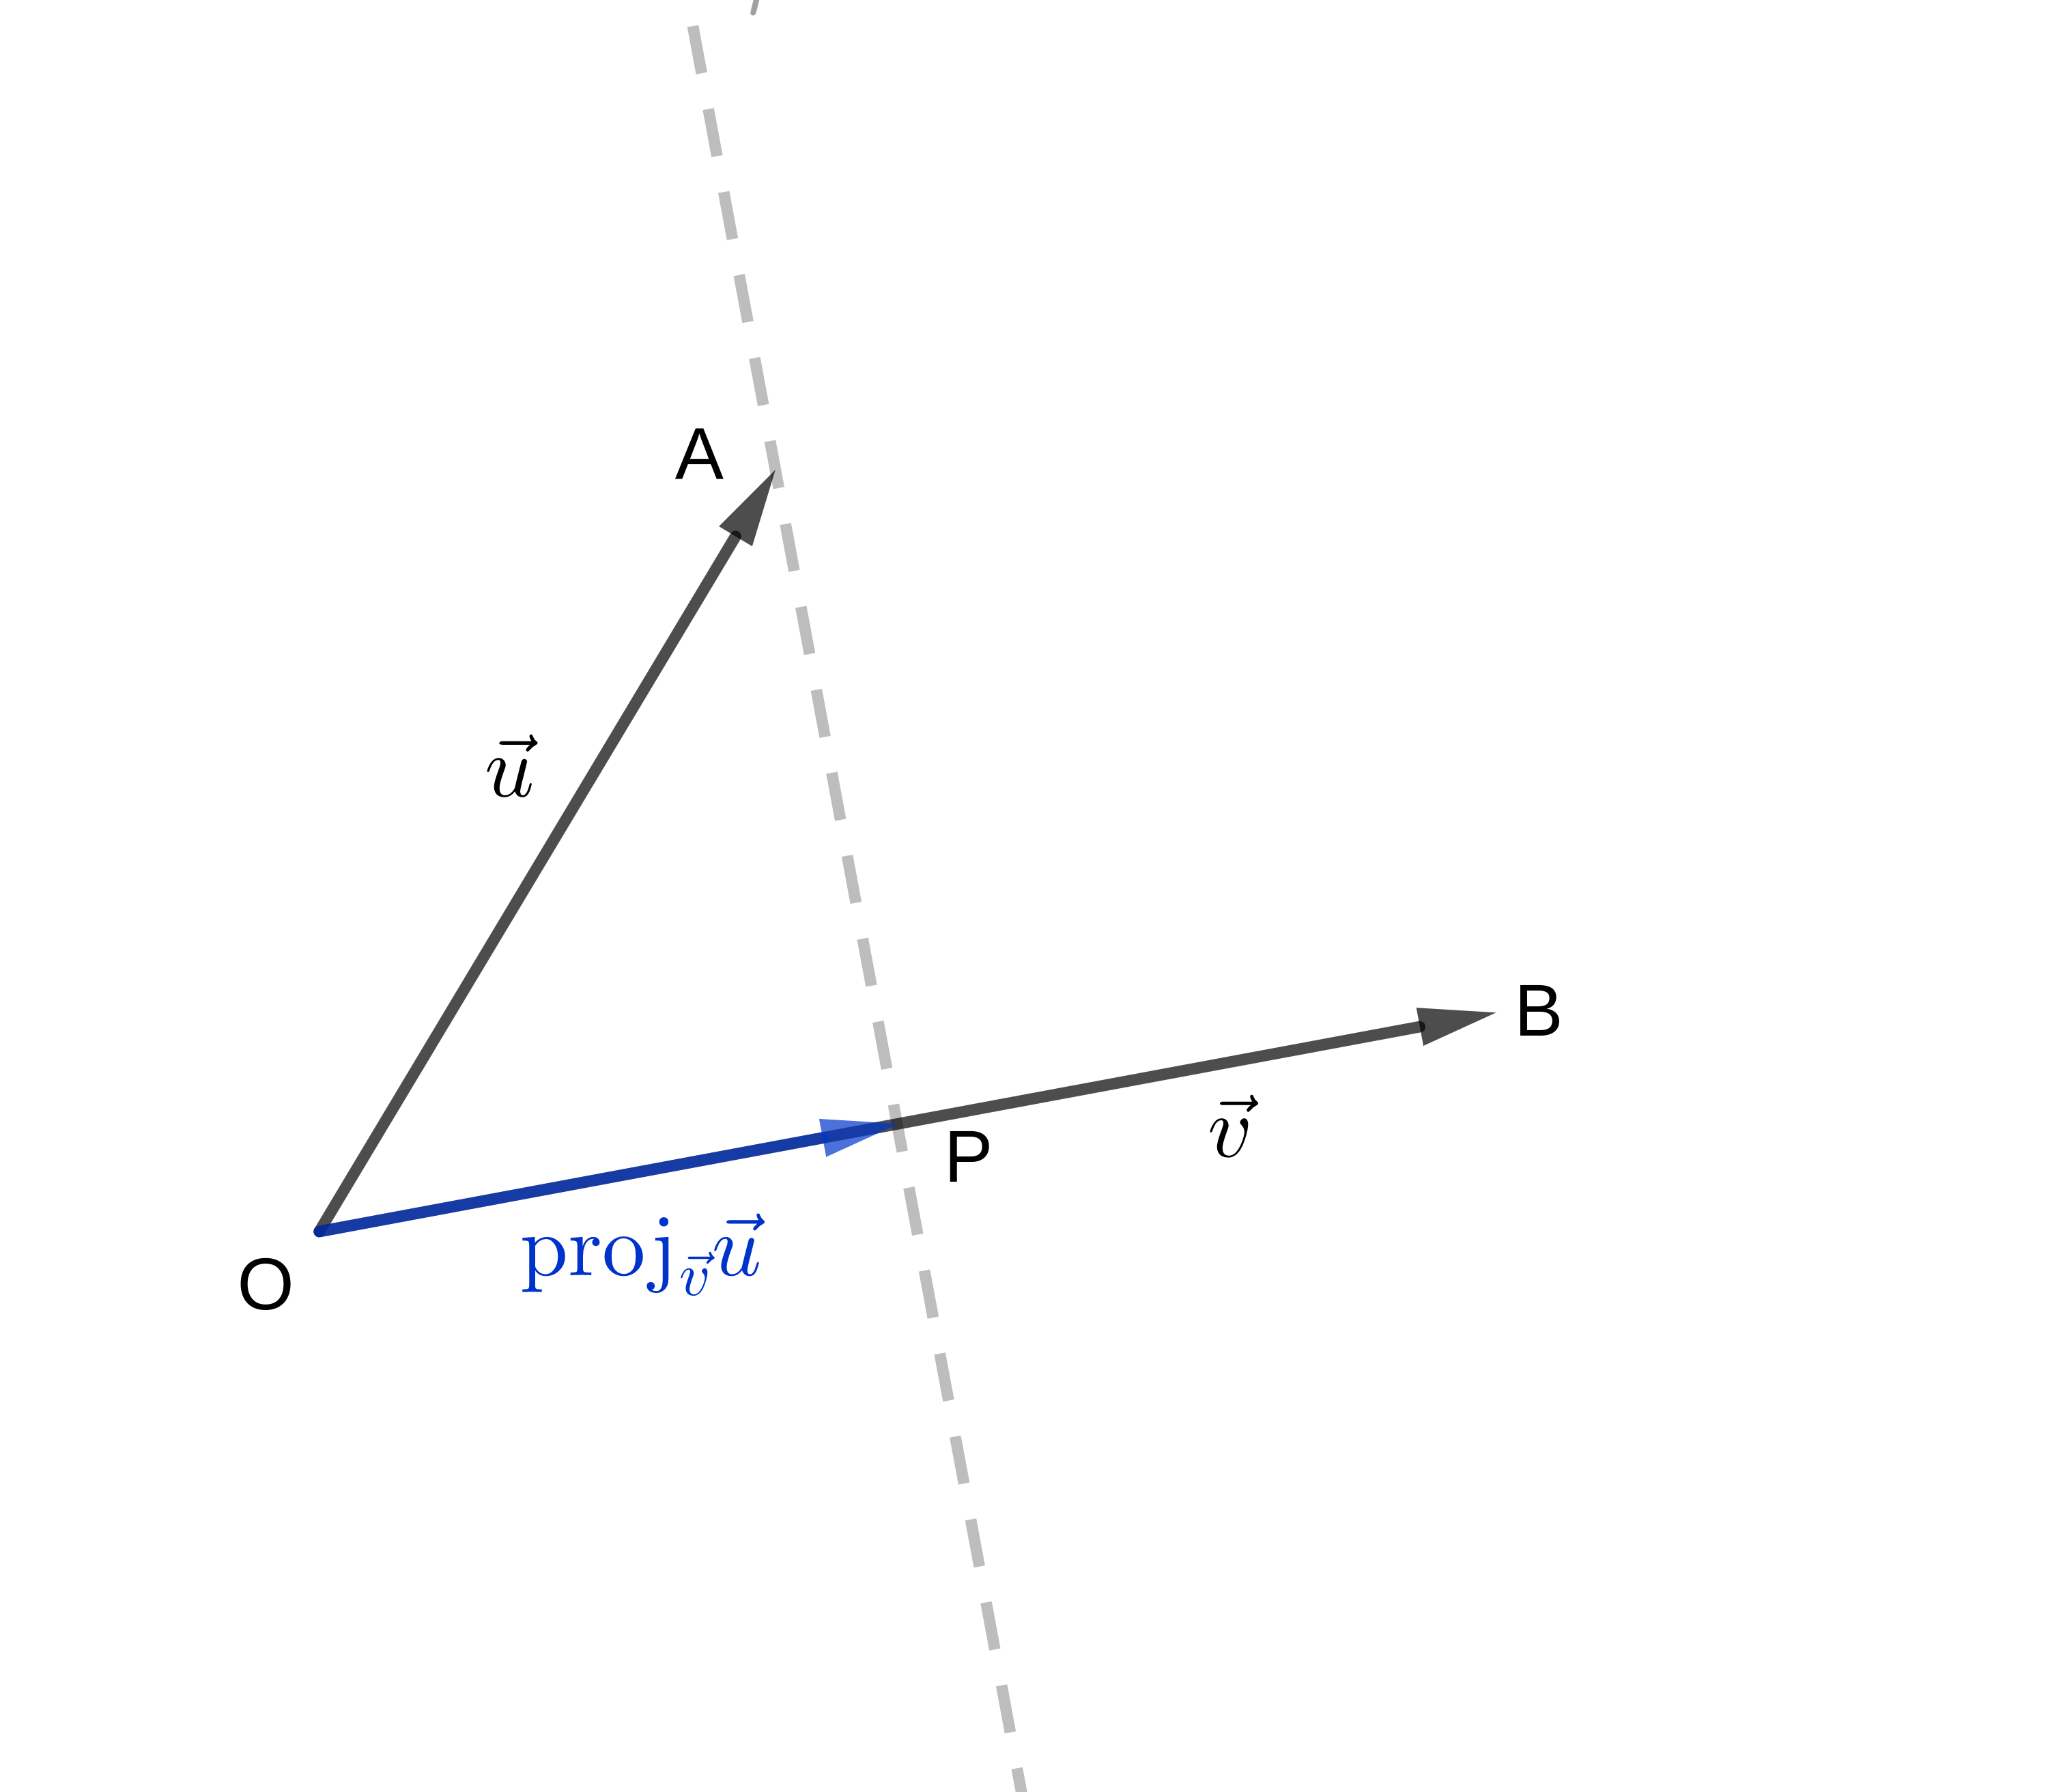
\includegraphics[width=0.7\textwidth]{./cap_prodesc/dados/fig_proj/fig_proj}
  \caption{Ilustração da definição da projeção ortogonal.}
  \label{fig:proj}
\end{figure}

Da definição, temos que
\begin{equation}
  \proj_{\vec{v}}\vec{u} = \alpha\vec{v}
\end{equation}
para algum número real $\alpha$. Além disso, temos
\begin{equation}
  \proj_{\vec{v}}\vec{u} = \vec{u} + \overrightarrow{AP}.
\end{equation}
Portanto
\begin{equation}
  \alpha\vec{v} = \vec{u} + \overrightarrow{AP}.
\end{equation}
Tomando o produto escalar com $\vec{v}$ em ambos os lados desta equação, obtemos
\begin{equation}
  \alpha\vec{v}\cdot\vec{v} = \vec{u}\cdot\vec{v},
\end{equation}
pois $\overrightarrow{AP}\cdot\vec{v}=0$, uma vez que $\overrightarrow{AP}\perp\vec{v}$. Daí, lembrando que $\vec{v}\cdot\vec{v}=|v|^2$, temos
\begin{equation}
  \alpha = \frac{\vec{u}\cdot\vec{v}}{|\vec{v}|^2}
\end{equation}
e concluímos que
\begin{equation}\label{eq:proj}
  \proj_{\vec{v}}\vec{u} = \frac{\vec{u}\cdot\vec{v}}{|\vec{v}|^2}\vec{v}.
\end{equation}

\begin{ex}
  Sejam $\vec{u}=(-1,1,-1)$ e $\vec{v}=(2,1,-2)$. Usando a equação \eqref{eq:proj}, obtemos
  \begin{align}
    \proj_{\vec{v}}\vec{u} &= \frac{(-1,1,-1)\cdot(2,1,-2)}{|(2,1,-2)|^2}(2,1,-2)\\
                           &= \frac{-2+1+2}{4+1+4}(2,1,-2)\\
                           &= \left(\frac{2}{9},\frac{1}{9},\frac{-2}{9}\right).
  \end{align}
\end{ex}

\emconstrucao

\subsection*{Exercícios}

\emconstrucao